\documentclass[a4paper]{article}
\usepackage[francais]{babel}
\usepackage[utf8]{inputenc}

\usepackage{graphicx}
\usepackage{fancyhdr}
\usepackage{lastpage}
\usepackage{amsmath}
\usepackage{xspace}
\usepackage{textcomp}

\usepackage{hyperref}

\usepackage[top=30mm, bottom=30mm, left=25mm, right=25mm]{geometry}

\pagestyle{fancy}

\usepackage{helvet}
\usepackage{bbm}

\usepackage{verbatim}
\usepackage{amsmath}
\usepackage[table]{xcolor}
\definecolor{bleugris}{rgb}{.2,.4,.5}

\definecolor{colKeys}{rgb}{0,0,1} 
\definecolor{colIdentifier}{rgb}{0,0,0} 
\definecolor{colComments}{rgb}{0,0.5,1} 
\definecolor{colString}{rgb}{0.6,0.1,0.1} 

\usepackage{listings}

% Permet l'ajout de code par insertion du fichier le contenant
% Les arguments sont :
% $1 : nom du fichier à inclure
% $2 : le type de langage (C++, C, Java ...)
\newcommand{\addCode}[2]{%

  % Configuration de la coloration syntaxique du code
  \definecolor{colKeys}{rgb}{0,0,1}
  \definecolor{colIdentifier}{rgb}{0,0,0}
  \definecolor{colComments}{rgb}{0,0.5,1}
  \definecolor{colString}{rgb}{0.6,0.1,0.1}

  % Configuration des options 
  \lstset{%
    language = #2,%
    identifierstyle=\color{colIdentifier},%
    basicstyle=\ttfamily\scriptsize, %
    keywordstyle=\color{colKeys},%
    stringstyle=\color{colString},%
    commentstyle=\color{colComments},%
    columns = flexible,%
    %tabsize = 8,%
    showspaces = false,%
    numbers = left, numberstyle=\tiny,%
    frame = single,frameround=tttt,%
    breaklines = true, breakautoindent = true,%
    captionpos = b,%
    xrightmargin=10mm, xleftmargin = 15mm, framexleftmargin = 7mm,%
  }%
    \begin{center}
    \lstinputlisting{#1}
    \end{center}
}

\newcommand{\nTitle}[1]{%
	\clearpage
	\vspace*{\fill}		%
	\begin{center}	%
		\part{#1}		%
	\end{center}
	\vspace*{\fill}		%
	\clearpage
}

\newenvironment{nAbstract} 		%
{ 								%
	\newpage 					% 
	\vspace*{\fill}				%
	\begin{center}			 	%
		\begin{abstract}		%
}{								%
		\end{abstract}			%
	\end{center}				%
	\vspace*{\fill}				%
	\newpage					%
}


\newcommand{\nClass}[1]{{\color{bleugris}{\textsl{\textbf{#1}}}}}
\newcommand{\nParameter}[1]{{\color{gray}{\textbf{#1}}}}
\newcommand{\nMethod}[1]{{\color{gray}{\textbf{#1}}}}
\newcommand{\nConstant}[1]{\texttt{\uppercase{#1}}}
\newcommand{\nKeyword}[1]{\textsl{\textbf{#1}}}

\graphicspath{{../SourcesMatlab/}}

% Conversion nombres arabes / romain
\makeatletter
\newcommand{\rmnum}[1]{\romannumeral #1}
\newcommand{\Rmnum}[1]{\expandafter\@slowromancap\romannumeral #1@}
\makeatother

\setlength{\headheight}{14pt}

\fancyhf{}


\makeatletter
\def\clap#1{\hbox to 0pt{\hss #1\hss}}%
\def\ligne#1{%
\hbox to \hsize{%
\vbox{\centering #1}}}%
\def\haut#1#2#3{%
\hbox to \hsize{%
\rlap{\vtop{\raggedright #1}}%
\hss
\clap{\vtop{\centering #2}}%
\hss
\llap{\vtop{\raggedleft #3}}}}%
\def\bas#1#2#3{%
\hbox to \hsize{%
\rlap{\vbox{\raggedright #1}}%
\hss
\clap{\vbox{\centering #2}}%
\hss
\llap{\vbox{\raggedleft #3}}}}%
\def\maketitle{%
\thispagestyle{empty}\vbox to \vsize{%
\vfill
\vspace{1cm}
\begin{flushleft}
\usefont{OT1}{ptm}{m}{n}
\huge \@title
\end{flushleft}
\par
\hrule height 4pt
\par
\begin{flushright}
\usefont{OT1}{phv}{m}{n}
\Large \@author
\par
\end{flushright}
\vspace{1cm}
\vfill
\vfill
\bas{}{\@blurb \vspace{1cm}}{}
}%
\cleardoublepage
}
\def\date#1{\def\@date{#1}}
\def\author#1{\def\@author{#1}}
\def\title#1{\def\@title{#1}}
\def\blurb#1{\def\@blurb{#1}}
\author{}
\title{}
\blurb{}
\makeatother


\usepackage{hyperref}
\hypersetup{
colorlinks=false, % bool: Liens colorés
pdfborder={0 0 0} % Ne pas encadrer les liens
}

\usepackage[final]{pdfpages}
\usepackage{rotating}
\usepackage{eurosym}
\usepackage{lscape}
\usepackage{float}
\usepackage{color}
\usepackage{colortbl}
\usepackage[printonlyused]{acronym}

% définir les commandes ici

% s'il y a beaucoup de commandes et de packages à inclure n'h&ésitez pas
% à mettre tout ça dans un fichier include.tex et l'inclure
% \input{include.tex}

\lhead{PdC2 - Dossier d'Architecture}
\rhead{
\includegraphics [width=1.5cm]{insa-couleur.jpg}}
\rfoot{\thepage\ de \pageref{LastPage}}



\begin{document}
\title{PdC 2 : Architecture technique détaillée}
\author{Elisa ABIDH, Adrien BROCHOT, Martin RICHARD, Jetmir XHEMBULLA}

%------------------------------------- Page de titre
\maketitle
%\begin{titlepage}
%~

%\vfill
%\begin{Large}
%Septembre 2011
%\end{Large}
%\vfill
%\end{titlepage}
%----------------------------------------------------

%--------------------------------- Table des matières
\newpage
\tableofcontents
\newpage
%----------------------------------------------- Plan
\section{Analyse de l'existant}

Cette partie du dossier d'architecture technique a pour objectif de dresser un état des lieux de l'actuelle architecture réseau présente sur le campus de l'INSA de Lyon. Ce projet doit permettre d'effectuer une transition entre l'architecture actuelle et une nouvelle architecture gérant la ToIP. L'enjeu dans la gestion de ce projet est que le campus de l'INSA possède déjà un réseau optique complexe et gérant de nombreux bâtiments. La mise en place d'une nouvelle architecture ne devra pas engendrer des coupures prolongées dans les différents bâtiments.

\subsection{Etude Technique}

\subsubsection{Réseau téléphonique}

\paragraph{} Le réseau du campus utilise actuellement un réseau téléphonique analogique basé sur trois commutateurs internes (PABX). Le réseau téléphonique est donc actuellement complètement séparé du réseau de données et aucune gestion centralisée n'est installée pour contrôler ce réseau. Un réseau spécial pour les téléphones de secours a été mis en place afin d'être en mesure de contacter les services nécessaires en cas de sinistre sur le campus. Ces téléphones peuvent rester allumés jusqu'à 8 heures après une coupure de courant générale sur le campus. Ces téléphones sont analogiques également.

\paragraph{} D'autres services du campus comme les alarmes, les téléphones d'ascenseurs, et FAXs utilisent un réseau téléphonique analogique qu'il ne sera pas possible de passer en ToIP à cause de leur ancienneté ou des réglementation en vigueur. De plus, le contrat d'entretien des PABX est assuré jusqu'en 2014.


\subsubsection{Réseau de donnée}

\paragraph{} Le réseau de données de l'INSA doit fournir de nombreux services variés : de l'hébergement web, service d'authentification sur le réseau ROCAD, mail... Les équipements actuels sont très vétustes et les divers services actuels gérants le réseau ne connaissent pas la liste complète et l'emplacement des équipements installés dans les différents locaux. La vétusté du matériel entraine de nombreux problèmes diminuant la qualité de service et risquant une interruption de ce dernier en cas de défaillance critique. Les équipements sont souvent sur-exploités et atteignent jusqu'à 90\% de charge.

\paragraph{} Certains services critiques tels que la video surveillance passent également par ce réseau de donnée. Ces services ne peuvent pas s'effectuer dans la limite des contraintes de sécurité normales dans le réseau de donnée actuel.

\paragraph{} Les équipements passifs du réseau de donnée sont pour la plupart vieux d'une quarantaine d'année. La technologie utilisée est donc généralement dépassée et procure un service limité.

\paragraph{} Le campus dispose actuellement d'une unique boucle optique câblée à l'aide de fibre multimode ne permettant le débit gigabit que sur une distance de 500m. Elle représente le principal problème du réseau. Elle est au cœur de ce dernier et ne permet pas de remplir les contraintes de sécurité auxquelles ce réseau devrait être soumis. Il faut par conséquent prévoir son remplacement. les fourreaux actuels n'étant plus aux normes, il sera préférable de créer deux toutes nouvelles boucles optiques et veiller cette fois à prévoir les évolution future et garantir les possibilités d'évolutions futures. Cette boucle optique permet le transfert des données dans tout les campus jusqu'au bas de chaque bâtiment. le CISR en est l'actuel responsable.

\paragraph{} Pour les bâtiments intérieurs, la plupart disposent de plusieurs locaux techniques. Un fédérateur permet de transformer la liaison optique en Ethernet et répartir ensuite vers les différents locaux techniques les données. L'équipement actif est déjà en cours de rénovation par la DSI de l'INSA. Le but est encore une fois de rendre la maintenance de ces équipement plus facile et améliorer la qualité de service. L'équipement passif, quant à lui est à peu près maitrisé.

\paragraph{} Chaque service doit gérer son raccordement au local technique auquel il est raccordé (en général un local technique d'étage). Ceci entraine une grande disparité des équipements utilisés sur le réseau. Cette disparité rend l'ensemble du réseau difficile à maintenir : chaque équipement ayant un âge différent, un modèle différent...


\subsection{Etude organisationnelle}

\paragraph{• SIDD :} le Service Interuniversitaire du Domaine de la Doua s'occupe de piloter les prochains projets portés sur le campus et gère la maintenance extérieure.

\paragraph{• DIRPAT :} La Direction du Patrimoine, assure la maintenance des équipements et bâtiments du campus. Elle est également en charge des réseaux electriques.

\paragraph{• CISR :} le Centre Inter-établissements pour les Services Réseaux couvre à la fois l'université lyon 1 et l'INSA sur le campus de la Doua. Cette entité est divisée en 2 équipes : un équipe de 7 personnes qui gère les installation inter campus, qui est en charge des fibres présentes sur le campus. Elle n'a aucune autorité dans les bâtiments. La deuxième équipe est composée également de 7 personnes rattachées à l'université Lyon 1. Elle s'est occupé de la gestion des installations internes aux bâtiments des 14 campus, du déploiement de la ToIP et du réseau WIFI de l'Université Lyon 1.

\paragraph{• DSI :} Cette entité est directement rattachée à l'INSA, elle est en charge des équipements internes aux différents bâtiments reliés au réseau. Elle est en charge des équipements actifs et passifs dans les bâtiments, elle actuellement en phase de redéploiement d'équipements afin d'uniformiser les différents locaux techniques et de modernisr l'ensemble de l'infrastructure.

Il n'y a actuellement aucun outil de travail collaboratif et les échanges entre les différentes entités sont très variables. La DSI et la DIRPAT communiquent assez facilement, quelques relations non formelles se font entre la DSI et le CISR.


\subsection{Etude financière}

\paragraph{} Ce type de projet représentant un investissement conséquent pour le campus, il convient d'étudier la situation financière de la structure cible afin d'adapter notre solution à ses moyens actuels voire de repousser les dates des début de projet afin d'attendre un moment plus propice et éviter de sacrifier de la technique dans le seul but de gagner quelques années qui seront bien vite rattrapées si la maintenance de la nouvelle infrastructure pose des problèmes.

\paragraph{} L'INSA est actuellement dans une période de grande difficultés financières, la gestion financière étant précédemment quasi-inexistante, le retard accumulé dans cette gestion a plongé l'INSA dans de grands problèmes financiers. Une nouvelle équipe a récemment pris la tête de la gestion des finances et tente de changer les choses mais la route sera longue avant que tous les problèmes soient réglés.

\paragraph{} Les principales solutions adoptées étant les restrictions budgétaires, il sera dur de prouver l'intérêt du lancement de notre projet : l'informatique n'étant généralement pas considéré comme prioritaire dans ce genre de situation. Le réseau actuel fonctionne, presque, convenablement, sa rénovation risque de passer pour un luxe que l'école ne peut pas s'offrir. 

\paragraph{} Des partenariats avec certaines entreprises pourraient aider à faire baisser les prix de nombreux équipements, l'INSA a, par chance, un partenariat avec le constructeur cisco qui permettra certainement d'obtenir des prix assez bas pour les différents équipements nécessaires (switchs, équipements VoIP,...)

\paragraph{} De plus, actuellement, tous les raccordements au réseau de donnée du campus est à la charge de chaque service, aucun abonnement n'existe. Seul le téléphone nécessite un abonnement, indépendant. La création d'une nouvelle architecture modifiera la gouvernance du réseau avec pour objectif de centraliser cette gouvernance et permettra d'imposer un abonnement mensuel afin de mieux suivre les différents services et pouvoir plus simplement monitorer le réseau.






\subsection{Projets importants du campus}

\paragraph{} Le campus de l'INSA est en pleine phase de rénovation. C'est dans cette phase que s'inscrit le présent projet.

\paragraph{• Rénovation du réseau :} La DSI avait entrepris la rénovation des parties actives des équipements du campus mais en raison de la situation actuelle du budget de l'INSA, ce projet a été mis en pause.

\paragraph{• liaison entre Bat Jacquard et Bat Baconier :} Ces deux bâtiments sont les sièges respectivement de la DSI et du CISR, une liaison par fibre monomode doit être effectuée entre ces deux bâtiments.

\paragraph{• Plan Campus :} C'est un projet gouvernemental qui a pour but la rénovation des établissement d'enseignements supérieur afin de tous les remettre aux normes (electricité, eau, chauffage). Ce projet ne concerne pas les infrastructures réseau mais peut permettre d'utiliser les travaux dans le sol qu'il effectuera pour nous aider à déployer nos infrastructures.

\paragraph{• Réorganisation des services :} Une réorganisation des différents services de l'INSA est en cours, cette réorganisation bloque l'avancée de la rénovation car les différents services concernés par le déménagement refusent en général de payer la rénovation de leurs installation car ils sont sur le point de les quitter.




\newpage
\section{Modèles d'architecture}

\paragraph{} Le déploiement du réseau de téléphonie par IP sur le campus de
l'INSA ne peut être réalisé en rupture avec l'infrastructure analogique
existante à une telle échelle.
\paragraph{} La section qui suit décrira à un niveau conceptuel l'architecture
du réseau de téléphonie existant, de celui que nous proposons à terme, et de
celui que nous proposons durant la phase de transition.

\subsection{Architecture existante}
\paragraph{} L'architecture actuelle repose sur un PABX analogique chargé
d'effectuer la commutation des lignes et d'assurer la liaison vers le réseau
Numéris de l'opérateur.

\subsection{Architecture de transition}
\paragraph{} Todo

\subsection{Architecture cible}
\paragraph{} Todo


\newpage
\section{Logiciels utilisés}

\paragraph{} Cette section décrira les logiciels qui seront utilisés dans le
réseau ToIP dont nous décrivons l'architecture. Par logiciel, nous entendons
discuter des systèmes d'exploitation, protocoles, applications et composants
logiciels sur le serveur.

\paragraph{} Plusieurs critères de sélection on été retenus, les voici :
\begin{description}
	\item[Interopérabilité] Les outils retenus doivent être compatibles avec le
	réseau existant, qui est très hétérogène. Les logiciels doivent donc utiliser
	des standards ouverts tant que possible.
	\item[Popularité] La popularité d'une solution est un indicateur relativement
	fiable de sa pérennité, de la facilité d'accès à des informations et des
	compétences spécifiques pour l'utiliser.
	\item[Solution Open-Source] Nous pensons que les solutions Open-Source
	offrent généralement des bons niveau d'interopérabilité (ou à défaut, la
	possibilité de modifier ces produits) et permettent de réduire les coûts.
	Les solutions Open-Source sont par ailleurs moins souvent liées à du matériel
	spécifique.
	\item[Prix] Le prix des licences de logiciels est naturellement un facteur de
	décision important pour deux solutions offrant des caractéristiques similaires
	répondant à nos besoins.
	\item[Complexité de la solution] Une solution complexe est une solution
	difficile à déployer et à maintenir, et qui peut se révéler, à moyen
	terme, coûteuse ou difficile à rendre fiable.
\end{description}

\subsection{Protocoles et codecs}

\begin{description}
	\item[RTP et RTCP] Les protocoles \ac{RTP} et \ac{RTCP} sont des protocoles
	standards de communication en temps réel sur un réseau IP.
	\item[SIP] \ac{SIP} est un protocole standard ouvert couramment utilisé en
	téléphonie par IP. Il remplace progressivement le standard H.323, qui souffre
	de limitations techniques et de failles de sécurité connues. SIP permet
	également de gérer des sessions de visiophonie, de messagerie instantanée ou
	des communications en mode conférence (plus de deux interlocuteurs).
\end{description}

\subsection{Call Manager et passerelle IP}

\paragraph{} Nous envisageons d'utiliser la solution
Asterisk\footnote{\url{www.asterisk.org}}, qui répond très bien à nos critères
de sélection. C'est une solution Open-Source reconnue qui intègre un vaste panel
d'outil dédiés à la ToIP.

\paragraph{} Asterisk dispose de nombreuses fonctionnalités et d'un mécanisme
d'extensions très complet. Il est notamment compatible avec les protocoles
\ac{PRI} T0 et T1, pour se relier à une ligne analogique ou \ac{RNIS}. Cette
suite logicielle sera donc en mesure de supporter l'architecture de transition
et l'architecture cible sur un serveur disposant des interfaces matérielles
nécessaires.

\paragraph{} Asterisk sera déployé sur une distribution GNU/Linux d'entreprise
(type Redhat).

\subsection{Terminaux}

\paragraph{} Les autres équipements utiliseront généralement leurs firmwares
d'origine. Cependant, certains terminaux téléphonique pourront être remplacés
par des logiciels (clients SIP) installées sur un ordinateur si l'utilisateur le
souhaite. Cette configuration n'est pas évaluée dans le cadre de cette étude et
n'est pas recommandée, notamment pour des raisons de sécurité.

\newpage
\section{Matériel retenu}

\paragraph{} Cette section discute du matériel qui supportera l'infrastructure
du réseau ToIP sur le campus de l'INSA.

\paragraph{} Les principaux critères de sélection sont les suivants :
\begin{description}
	\item[Interopérabilité] Les outils retenus doivent être compatibles avec le
	réseau existant, qui est très hétérogène. Le matériel doit donc pouvoir
	travailler avec des produits commercialisés par la concurrence et permettre,
	si besoin, d'accueillir des cartes et interfaces réseau supplémentaires.
	\item[Prix] Le prix du matériel (à l'achat et pour la maintenance) sera
  déterminant, mais sera surtout discuté dans le cadre d'appels d'offres.
	\item[Popularité] La popularité d'une gamme est un indicateur sur
  l'interopérabilité du matériel et donne une bonne garantie sur sa pérennité.
\end{description}

\subsection{PABX}

\paragraph{} Le \ac{PABX} existant sera conservé lors de la phase de transition.
Nous veillerons à optimiser sa charge et nous assurer que les systèmes
d'alimentation de secours en place sont toujours pleinement opérationnels.

\subsection{Serveur}

\paragraph{} Nous optons pour un serveur garantissant une très haute
disponibilité et une fiabilité accrue. Le serveur sera équipée de technologies
matérielles conçues pour ces situations (RAID, fallbacks matériels, etc).

\paragraph{} Par ailleurs, ce serveur sera équipé d'interfaces réseau dédiées à
la connexion vers le réseau \ac{RNIS} ou analogique, telles que celles proposées
par la branche Hardware de la société Asterisk. Les cartes de la série Hx8 sont
des cartes hybrides disposant d'interfaces analogiques et numériques.

\paragraph{} Comme tout serveur critique, celui-ci est rattaché à un onduleur et
une alimentation de secours.

\paragraph{} Nous estimons le coût d'achat d'un tel serveur à 5000 \euro HT.

\subsection{Équipements coeur de réseau}

\paragraph{} Le matériel déployé au coeur du réseau sera généralement de la même
nature que celui déployé pour le reste du réseau IP du campus. D'une manière
générale, l'étude du matériel existant ou prévu à l'achat doit être reconsidéré
en tenant compte du surplus de trafic engendré par les postes de téléphonies par
IP envisagés dans le cadre de l'architecture cible.

\subsection{Switch POE}

\paragraph{} Les switchs qui doivent supporter le trafic de ToIP doivent être
équipés de technologies \ac{POE}, qui permet d'alimenter les terminaux
téléphoniques et éviter une interruption de service en cas de coupure
d'électricité. Ces switchs doivent être manageables (switchs de niveau 3) pour
permettre de créer des VLAN dédiés à la ToIP.

\paragraph{} Un switch POE accueille généralement une part de ports ethernet
équipés et des ports standards. Compte-tenu des investissements à prévoir de la
part de la DSI, nous pouvons envisager d'opter pour des switchs équivalents à
ceux qui sont prévus, mais disposant de l'option POE.

\paragraph{} Il faut noter que des switchs POE nécessitent des locaux équipés de
climatisation adaptée et un onduleur à batteries pour rester disponibles en cas
de panne d'alimentation.

\subsection{Téléphones IP}

\paragraph{} Les téléphones IP qui seront déployés doivent supporter les
protocoles que nous souhaitons utiliser, et principalement \ac{SIP}. La plupart
des terminaux du marchés sont compatibles avec une telle technologie.

\paragraph{} Les téléphones sont alimentés grâce à la téchnologie \ac{POE} et ne
nécessitent pas d'attention particulière pour garantir leur bon fonctionnement.

\newpage
\section{Définition des Boucles Optiques}

\paragraph{} Afin de déployer une nouvelle infrastructure réseau acceptant la ToIP dans le but de remplacer à terme l'ensemble des téléphones analogiques par des téléphones numériques (y compris les téléphones des secours), il est nécessaire de pouvoir assurer le transfert de données en toute circonstances. La sécurité du réseau doit être assurée par une double connexion de chaque bâtiment au réseau optique du campus. De cette manière, même en cas de défaillance d'une fibre, les données pourront toujours circuler. L'unique boucle optique actuellement disponible sur le campus ne répond pas aux exigences de sécurité citées ci-dessus. Elle est également déployée dans des fourreaux anciens et ne répondant pas aux normes de sécurité actuelles. Enfin, les fibres sont principalement des fibres optiques multimode ne permettant pas un débit suffisant pour gérer à la fois le réseau de données et le réseau téléphonique qui devront passer par les mêmes voies.

\paragraph{} De grands travaux d'aménagement seront effectués lors de la mise en place du projet de déploiement de ToIP sur le campus. Deux nouvelles connexions de fibres optiques seront mises en place : une boucle et une étoile. Ces connexion seront installées dans de nouveaux fourreaux enterrés dans tout le campus. Nous utiliserons des fibres monomodes, les nouvelles connexions formeront un réseau permettant à chaque bâtiment d'avoir deux accès indépendants au réseau global du campus. Les figures ci-dessous présentent les deux connexions avec les nœuds optiques associés.

\paragraph{} Les boucles seront créées selon un schéma de déploiement en étoile autour du bâtiment Jacquard qui représente le cœur du réseau. La boucle (qui est la connexion principale) est en plus conçue pour transporter les données d'un nœud à l'autre même en cas de section d'une partie de la boucle.


\begin{figure}[h]
  \caption{\label{Plan_boucle1} Première boucle optique}
  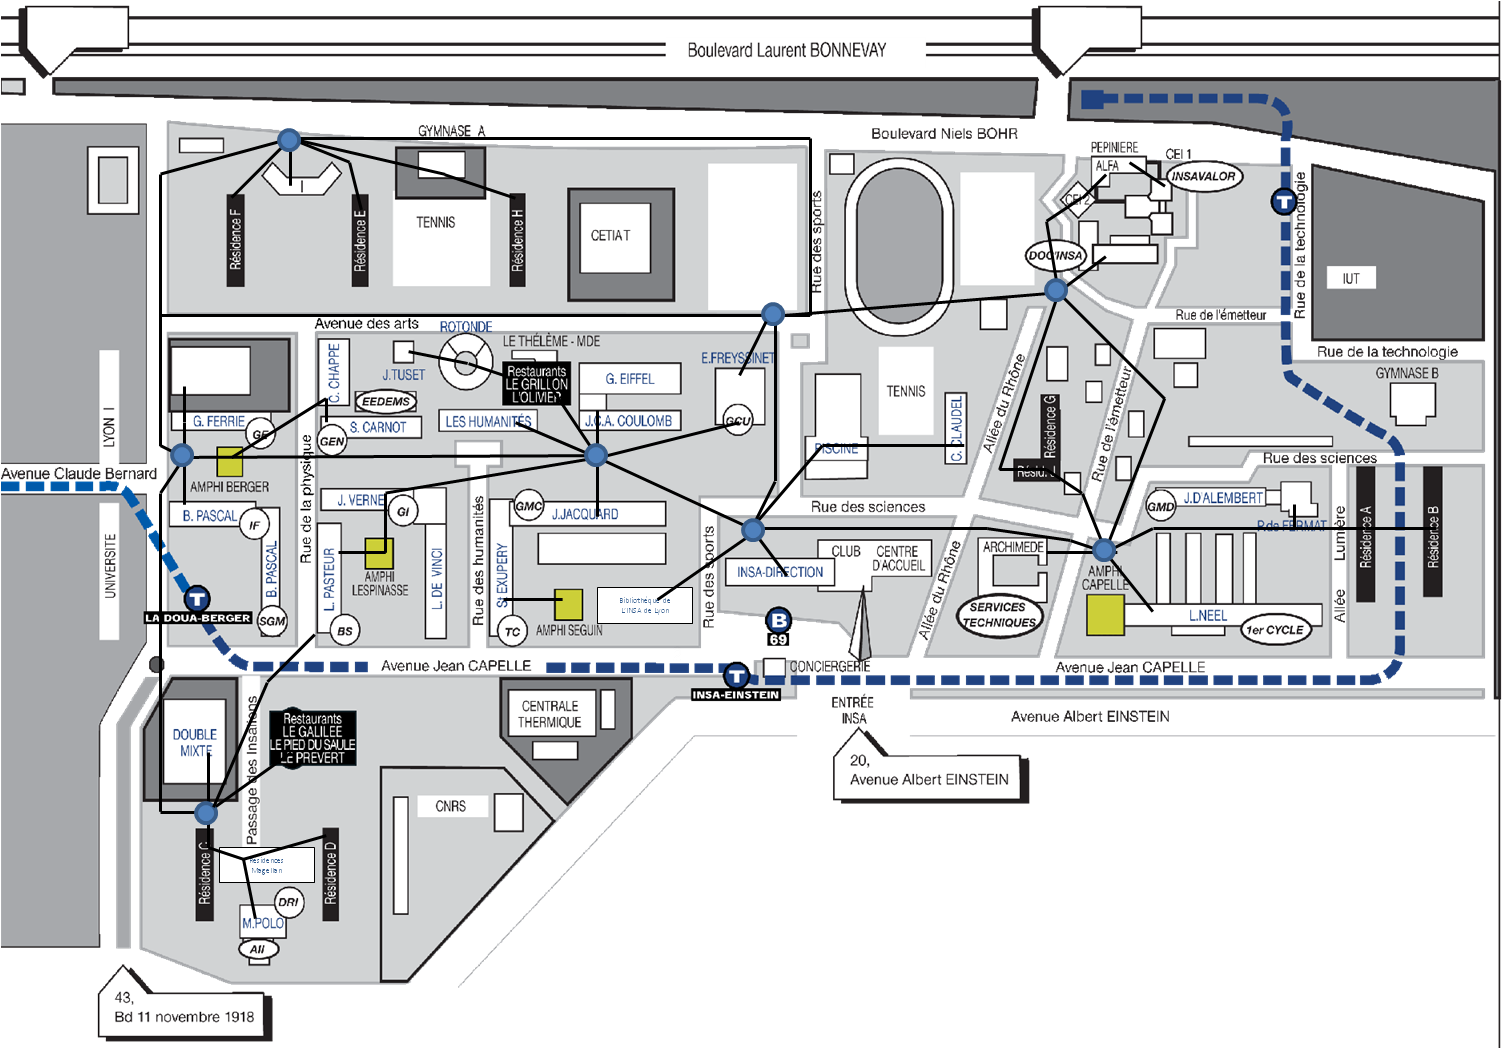
\includegraphics[scale=0.6]{Boucle1.png}
\end{figure}

\begin{figure}[h]
  \caption{\label{Plan_boucle2} Deuxième boucle optique}
  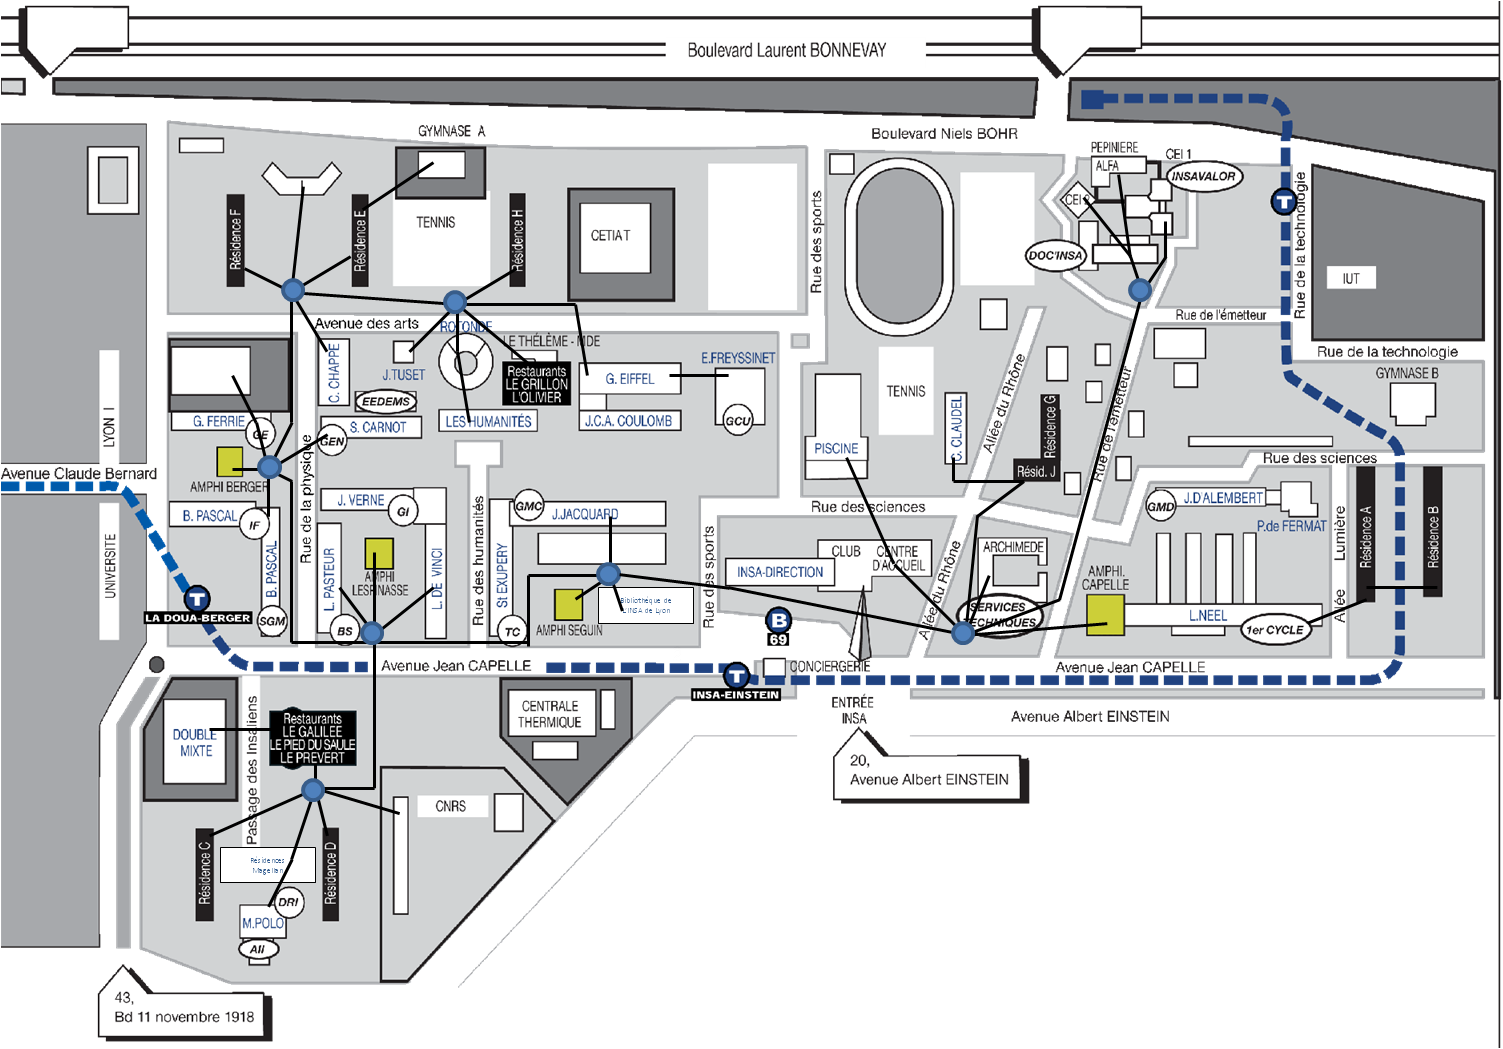
\includegraphics[scale=0.6]{Boucle2.png}
\end{figure}
~\\

\paragraph{} Nous pouvons remarquer que le déploiement de ces boucles conduira à la construction de 16 nœuds optiques et entrainera la pose de 6000 mètres de fourreaux pour la boucle 1 et 4500 mètres pour la seconde. Ces nœuds seront les points de convergence des fourreaux. L'alimentation électrique de ces nœuds se fera par câbles électriques enterrés dans des fourreaux parallèles aux fourreaux de fibre optique. Cette connexion permettra non seulement de n'avoir à effectuer qu'une seule tranchée pour les fibres et l'alimentation mais également de permettre de centraliser l'alimentation des différents nœuds et locaux techniques au bâtiment Jacquard ce qui permettra d'y installer les équipements de protection en cas de coupure de courant sur le campus (onduleur sur batterie, groupe électrogène).

\paragraph{} Deux chambres de tirage de fibre optique seront créées par bâtiment raccordé au boucles (une par connexion). Ces deux chambres de tirage raccorderont chaque bâtiment par deux emplacements distincts et espacés géographiquement afin de réduire les risques de déconnexion des bâtiments en cas de sinistre dans une partie de celui-ci.

\paragraph{} Comme présenté dans les plans, les fourreaux seront placés entre les bâtiments connectés. Afin de limiter le nombre de nœuds optiques, certaines fibres passeront à l'intérieur d'un bâtiment et seront redirigées vers un autre fourreau de sortie dans le local technique de ce dernier pour connecter un bâtiment voisin. Afin de prévenir de tout risque causé par le destruction de fourreaux aux abords des locaux techniques, chaque bâtiment connecté au réseau disposera de deux points d'entrées bien distincts pour les connexions des deux boucles optiques (en général : un point d'entrée pour la première boucle au niveau du local technique, une deuxième point d'entrée pour la seconde à l'autre bout du bâtiment. La fibre sera amenées au local par le câblage interne du bâtiment).

\paragraph{} La plupart des bâtiments du campus sont déjà équipés de locaux techniques pour la gestion de leur parc informatique. Lors de la mise en place des fourreaux pour la connexion d'un bâtiment, ces locaux techniques seront rénovés et équipés avec le matériel nécessaire à la gestion des deux nouvelles connexions. La rénovation passera par le changement des switchs qui seront utilisés par les téléphones en switchs POE, l'installation de climatisation dans les locaux (les switchs POE émettent plus de chaleur en fonctionnement que les switchs normaux), la création des deux nouvelles chambres de tirage décrites ci-dessus.

\paragraph{} Si la place disponible dans les locaux techniques d'un bâtiment n'est pas suffisante, de nouveaux locaux pourront être créés après destruction des anciens. La politique sera alors la création d'un ou deux locaux techniques par bâtiment (en fonction de la taille de ce dernier). Ce locaux techniques seront situés le plus possible aux étages médians des bâtiments afin de limiter la longueur des câbles Ethernet dans les bâtiments. 
\newpage
\section{Acronymes utilisés dans ce document}

\begin{acronym}
  \acro{PABX}{Private Automatic Branch eXchange}
  \acro{POE}{Power Over Ethernet}
	\acro{PRI}{Primary Rate Interface}
  \acro{RNIS}{Réseau numérique à intégration de services}
	\acro{RTCP}{Real Time Control Protocol}
	\acro{RTP}{Real Time Protocol}
	\acro{SIP}{Session Initiation Protocol}
\end{acronym}

%\newpage
%\input{Reseau.tex}
%\newpage

\end{document}
